%%%%%%%%%%%%%%%%%%%%%%%%%%%%%%%%%%%%%%%%%%%%%%%%%%%%%%%%%%%%%%%%%%%%%%%%%%%%%%%
% Preamble
%%%%%%%%%%%%%%%%%%%%%%%%%%%%%%%%%%%%%%%%%%%%%%%%%%%%%%%%%%%%%%%%%%%%%%%%%%%%%%%
\documentclass[aspectratio=169]{beamer}

% Packages
\usepackage{amsthm}
\usepackage{amssymb}
\usepackage{amsfonts}
\usepackage{amsmath}
\usepackage{mathtools}
\usepackage{pgf}
\usepgflibrary{fpu}
\usepackage{pgfplots}
\usepackage{tikz}
\usetikzlibrary{angles,fit,arrows,calc,math,matrix,intersections,through,backgrounds}
\usepackage{tikz-cd}
\usepackage{tkz-euclide}
\usepackage{tkz-graph}
\usepackage{graphicx}
\usepackage{hyperref}
\pgfplotsset{compat=1.18}

% Theme
\usetheme{Pittsburgh}
\usecolortheme{seahorse}

% Title and Author
\title{Arithmetic Expression Geometry:\\Five Possibilities}
\author[Mingli Yuan]{Mingli Yuan}
\date{\today}

\begin{document}

%%%%%%%%%%%%%%%%%%%%%%%%%%%%%%%%%%%%%%%%%%%%%%%%%%%%%%%%%%%%%%%%%%%%%%%%%%%%%%%
% Title and Introduction
%%%%%%%%%%%%%%%%%%%%%%%%%%%%%%%%%%%%%%%%%%%%%%%%%%%%%%%%%%%%%%%%%%%%%%%%%%%%%%%

\begin{frame}
    \maketitle
\end{frame}

\begin{frame}
    \frametitle{Table of Contents}
    \tableofcontents
\end{frame}

%%%%%%%%%%%%%%%%%%%%%%%%%%%%%%%%%%%%%%%%%%%%%%%%%%%%%%%%%%%%%%%%%%%%%%%%%%%%%%%
%
%%%%%%%%%%%%%%%%%%%%%%%%%%%%%%%%%%%%%%%%%%%%%%%%%%%%%%%%%%%%%%%%%%%%%%%%%%%%%%%

\section{Foreword: A few small, colorful stones}

\begin{frame}
    \frametitle{Foreword: A few small, colorful stones}
        \begin{columns}
        \begin{column}{0.55\textwidth}
Over the past ten years of exploration, I’ve collected a few small, colorful stones.
\newline\newline
Each one sparked my curiosity, and together they have carried me to where I am today.
\newline\newline
The stones are not answers, but invitations — to keep exploring, to keep asking, and to enjoy the process.
\newline\newline
Asking the right questions is often more important than finding the right answers, especially in the AI era.
        \end{column}
        \begin{column}{0.45\textwidth}
            \begin{figure}[ht]\centering
                \resizebox{0.7\textwidth}{!}{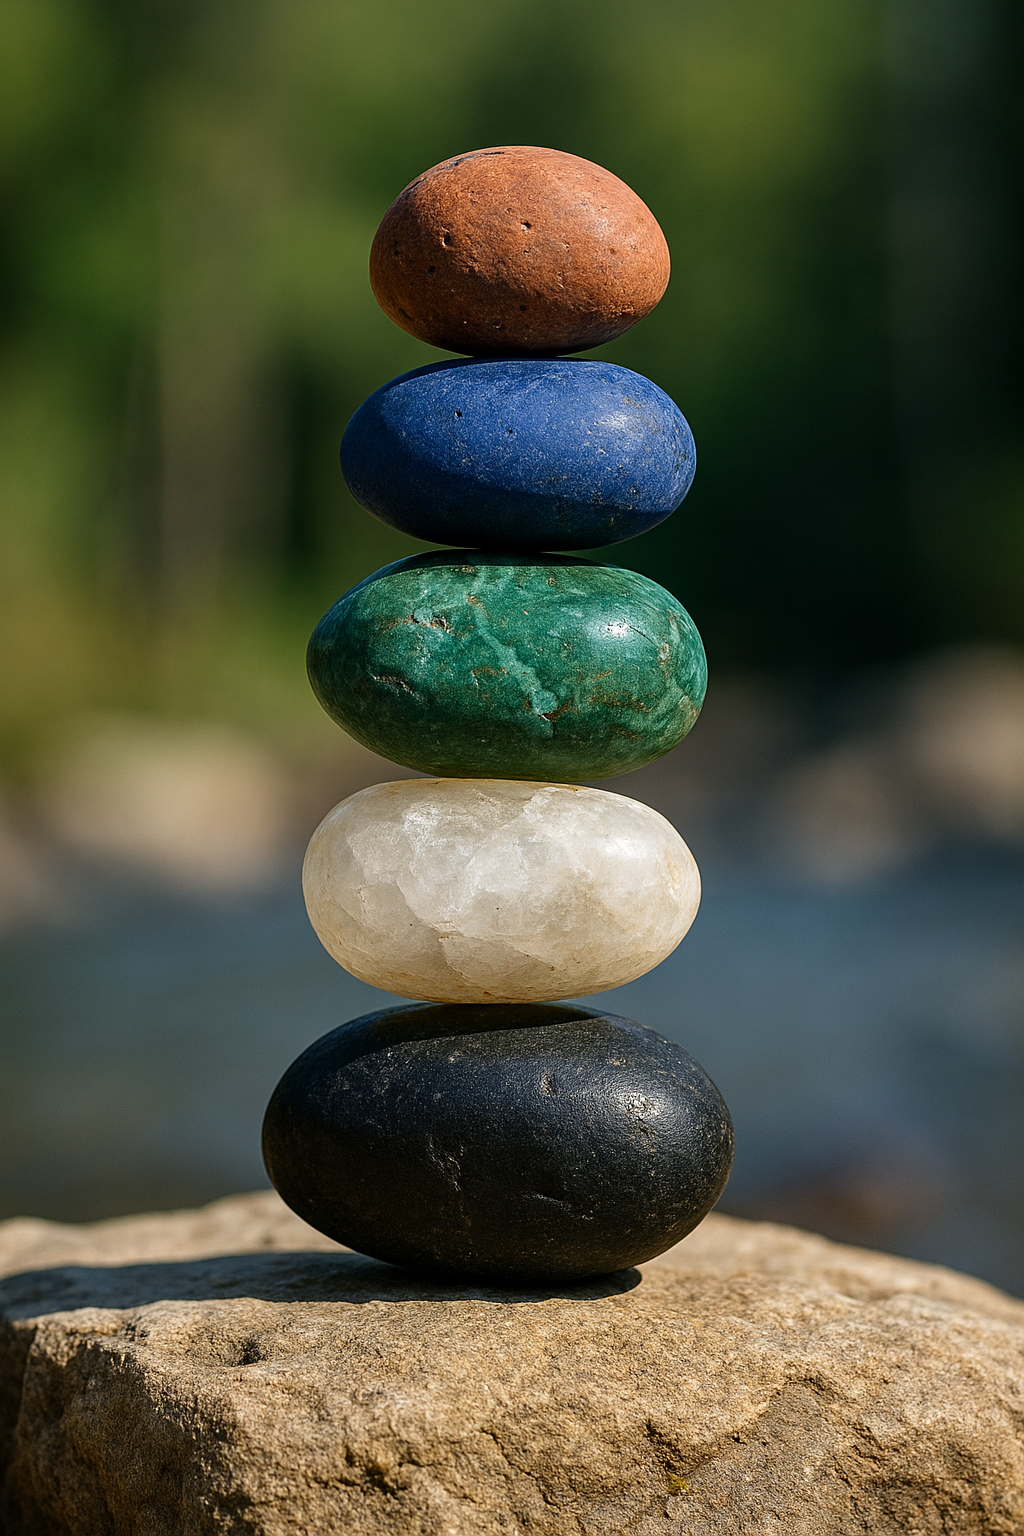
\includegraphics{../images/rock_balancing}}
            \end{figure}
        \end{column}
    \end{columns}

\end{frame}

%%%%%%%%%%%%%%%%%%%%%%%%%%%%%%%%%%%%%%%%%%%%%%%%%%%%%%%%%%%%%%%%%%%%%%%%%%%%%%%
% Possibility 1: From Non-commutativity to Complexity
%%%%%%%%%%%%%%%%%%%%%%%%%%%%%%%%%%%%%%%%%%%%%%%%%%%%%%%%%%%%%%%%%%%%%%%%%%%%%%%

\section{Ochre: The red stone of beginnings}

\begin{frame}
    \frametitle{Ochre: The red stone of beginnings}
    \begin{center}
        \Large
        \textbf{From Non-commutativity to Complexity}\newline\newline
        \emph{How does non-commutativity lead to complexity, and how can we geometrize it?}
    \end{center}
\end{frame}

\begin{frame}
\frametitle{Regularity of word2vec}
A well-known example is word2vec:

\begin{itemize}
    \item Parallelism encodes semantic analogy: concepts are points, relations are vectors.
    \item However, this regularity is not fully or rigorously enforced in word2vec. What happens if we enforce it strictly?
\end{itemize}
\begin{figure}[ht]
\centering
\resizebox{0.5\textwidth}{!}{
\begin{tikzpicture}[x=0.5cm,y=0.5cm,z=0.3cm,>=stealth]
\draw[->] (xyz cs:x=-7.0) -- (xyz cs:x=7.0) node[above] {$x_0$};
\draw[->] (xyz cs:y=0) -- (xyz cs:y=7.0) node[right] {$x_n$};
\draw[->] (xyz cs:z=-7.0) -- (xyz cs:z=7.0) node[above] {$x_i$};

\node[fill,circle,inner sep=1.5pt,label={left:$king$}] (p) at (xyz cs:x=-3.0, y=3.0, z=-3.0) {};
\node[fill,circle,inner sep=1.5pt,label={right:$man$}] (q) at (xyz cs:x=2.0, y=-3.0, z=3.0) {};
\node[fill,circle,inner sep=1.5pt,label={left:$queen$}] (r) at (xyz cs:x=-3.0, y=3.0, z=3.0) {};
\node[fill,circle,inner sep=1.5pt,label={right:$woman$}] (s) at (xyz cs:x=2.0, y=-3.0, z=9.0) {};
\draw[dashed, blue] (p) -- (q);
\draw[dashed, blue] (r) -- (s);
\draw[dashed, red] (p) -- (r);
\draw[dashed, red] (q) -- (s);
\end{tikzpicture}
}
\caption{Regularity in word2vec}
\label{fig:regularity-of-word2vec}
\end{figure}
\end{frame}

\begin{frame}
\frametitle{The case of numbers}
\[
(\alpha + 1) \times 2 \neq \alpha \times 2 + 1
\]

\begin{itemize}
    \item First-class elements: numbers (points), operations (generators), and relationships (operation sequences/paths) are modeled explicitly.
    \item Regularity strictly enforced: the same operation sequence induces the same geometric displacement; different orders encode different relationships.
    \item Both ``relationship'' and ``concept'' are treated as first-class, fully consistent with this regularity.
\end{itemize}

\begin{figure}[ht]
\centering
\resizebox{0.5\textwidth}{!}{
\begin{tikzpicture}[x=0.5cm,y=0.5cm,z=0.3cm,>=stealth]
\draw[->] (xyz cs:x=-7.0) -- (xyz cs:x=7.0) node[right] {$x_0$};
\draw[->] (xyz cs:y=0) -- (xyz cs:y=7.0) node[right] {$x_n$};
\draw[->] (xyz cs:z=-7.0) -- (xyz cs:z=7.0) node[above] {$x_i$};

\node[fill,circle,inner sep=1.5pt,label={left:$\alpha$}] (p) at (xyz cs:x=-3.0, y=3.0, z=-3.0) {};
\node[fill,circle,inner sep=1.5pt,label={right:$\alpha+1$}] (q) at (xyz cs:x=2.0, y=-3.0, z=3.0) {};
\node[fill,circle,inner sep=1.5pt,label={left:$\alpha \times 2$}] (r) at (xyz cs:x=-3.0, y=3.0, z=3.0) {};
\node[fill,circle,inner sep=1.5pt,label={right:$(\alpha + 1) \times 2 \neq \alpha \times 2 + 1$}] (s) at (xyz cs:x=2.0, y=-3.0, z=9.0) {};
\draw[dashed, blue] (p) -- (q);
\draw[dashed, blue] (r) -- (s);
\draw[dashed, red] (p) -- (r);
\draw[dashed, red] (q) -- (s);
\end{tikzpicture}
}
\caption{Non-commutativity of operations in Euclidean space}
\label{fig:noncommutativity-numbers}
\end{figure}
\end{frame}

\begin{frame}
    \frametitle{Explosion of symbolic combinations}
    \begin{columns}
        \begin{column}{0.55\textwidth}
            \begin{itemize}
                \item Once non-commutativity is introduced, the number of distinct operation strings grows \emph{exponentially}.
                \item Generation trees visualize this explosion: greater depth leads to a combinatorial surge in distinct expressions.
                \item Intuition: branching factor $>1$ implies exponential growth.
            \end{itemize}
        \end{column}
        \begin{column}{0.45\textwidth}
            \begin{figure}[ht]\centering
                \resizebox{0.9\textwidth}{!}{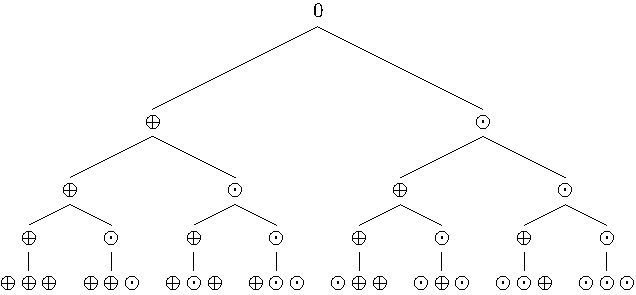
\includegraphics{../images/explosion}}
                \caption{Tree expansion of possible generation sequences}
            \end{figure}
        \end{column}
    \end{columns}
\end{frame}

\begin{frame}
    \frametitle{From symbols to geometry: hyperbolicity and volume}
    \begin{itemize}
        \item Assume each operation sequence maps to a point in a geometric space, and that balls of radius $\delta$ have uniformly positive volume.
        \item Then the symbolic explosion caused by non-commutativity corresponds to exponential growth of volume.
        \item Hyperbolic spaces exemplify this behavior:
        \[
            \mathrm{Vol}(B_r) \sim e^{(n-1)r}
        \]
    \end{itemize}
    \begin{columns}
        \begin{column}{0.3\textwidth}
            \begin{figure}[ht]\centering
                \resizebox{0.9\textwidth}{!}{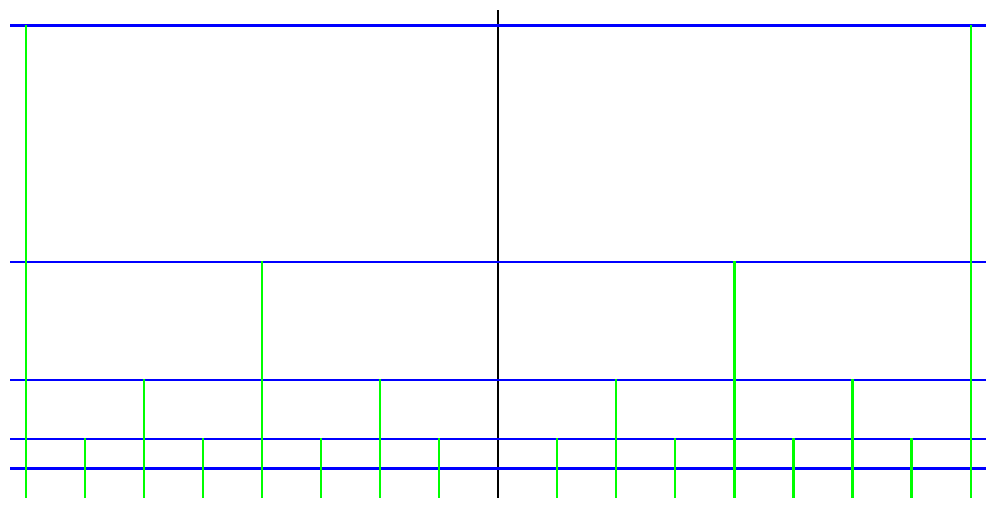
\includegraphics{../images/non-parallelogram}}
                \caption{Non-parallelogram $\Rightarrow$ hyperbolicity}
            \end{figure}
        \end{column}
        \begin{column}{0.3\textwidth}
            \begin{figure}[ht]\centering
                \resizebox{0.5\textwidth}{!}{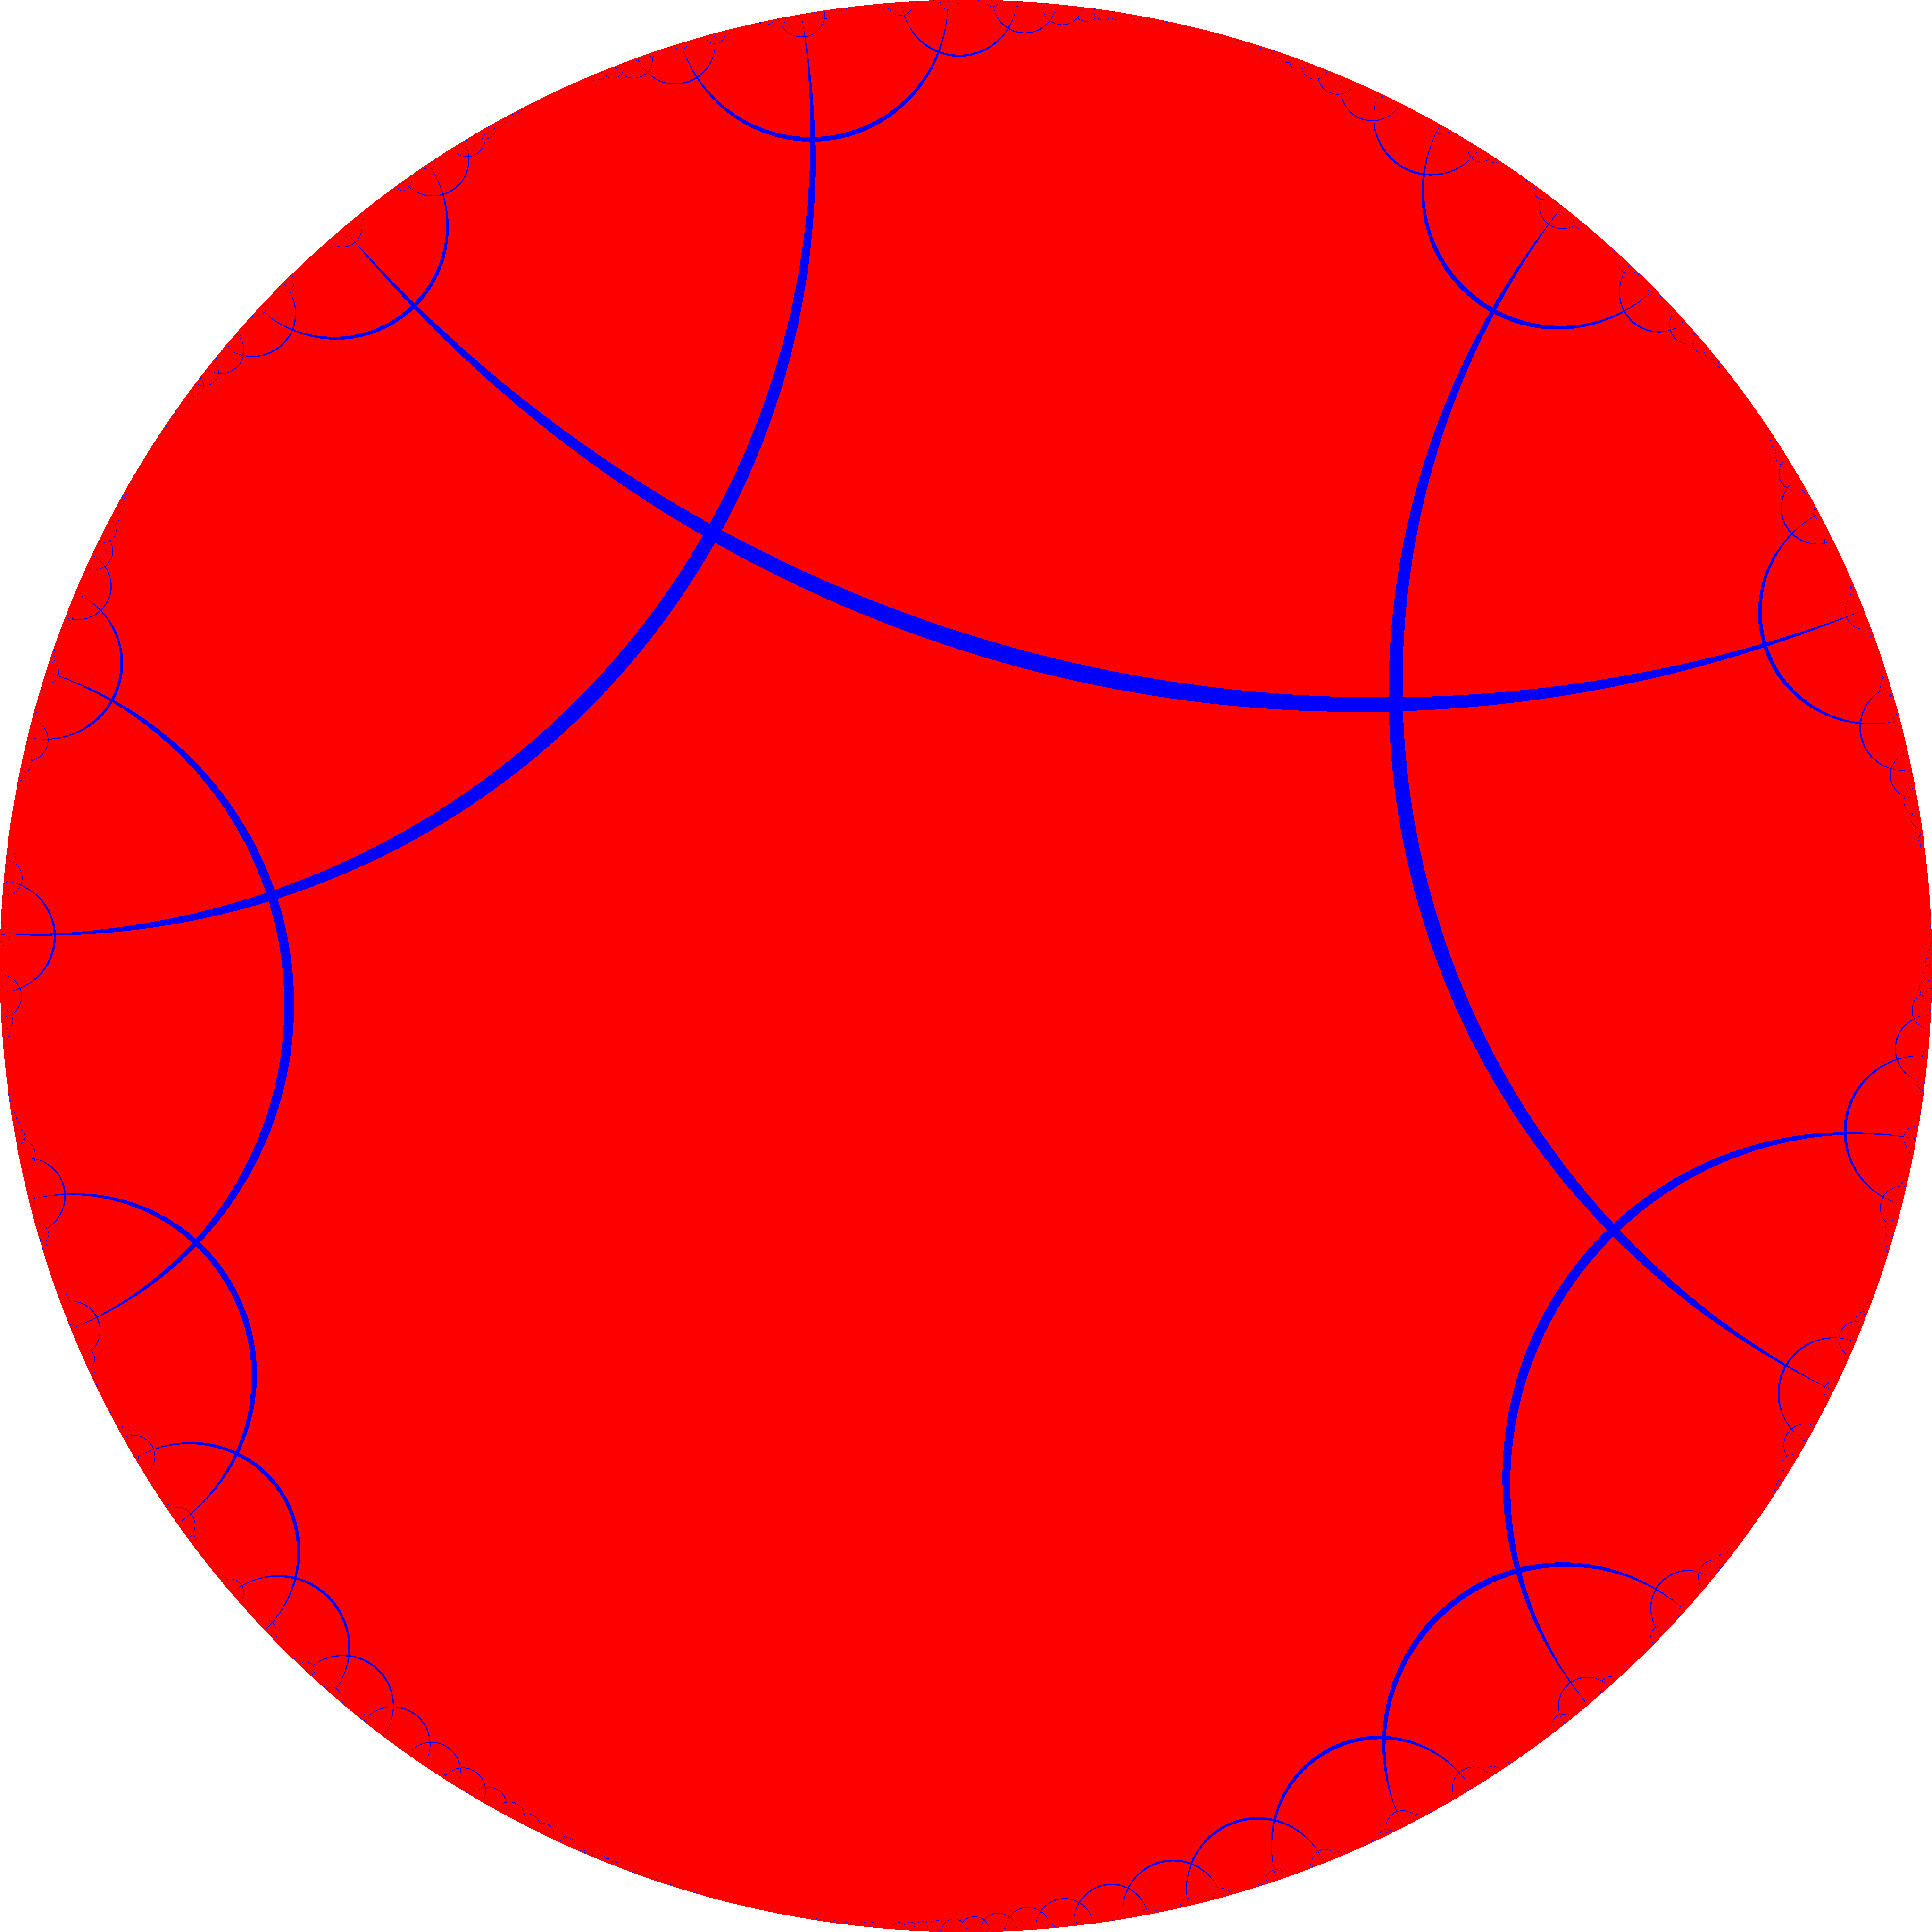
\includegraphics{../images/t4096}}
                \caption{A hyperbolic tessellation}
            \end{figure}
        \end{column}
    \end{columns}
\end{frame}

\begin{frame}
    \frametitle{Contrast: the linear/commutative case}
    \begin{itemize}
        \item If operations commute or are constrained by linearity, the \emph{parallelogram law} holds.
        \item The parallelogram law simplifies the generation process and mitigates the explosion of symbolic combinations.
        \item Euclidean ball volume: $\mathrm{Vol}(B_r) \propto r^n$ (polynomial in $r$).
    \end{itemize}
    \begin{figure}[ht]\centering
        \resizebox{0.5\textwidth}{!}{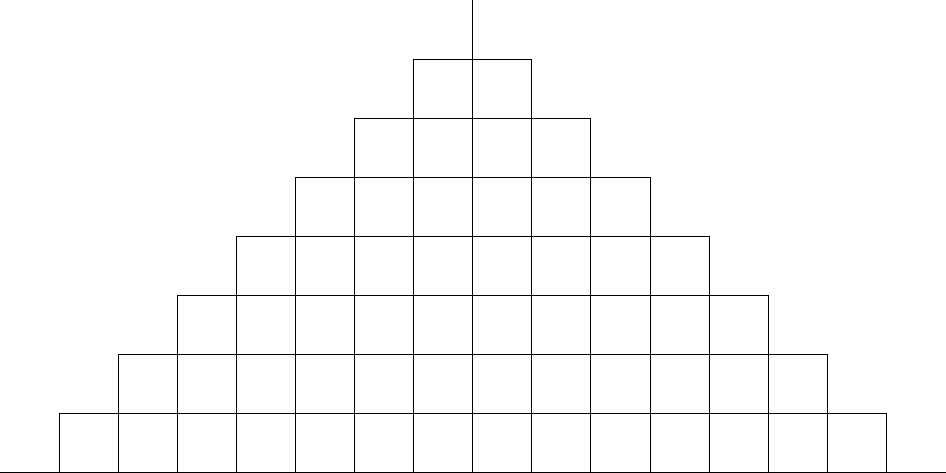
\includegraphics{../images/parallelogram}}
        \caption{Parallelogram law $\Rightarrow$ Euclidean linearity}
    \end{figure}
\end{frame}

\begin{frame}
    \frametitle{Conclusion: complexity as a geometric volume}
    We have shown that:
    \begin{itemize}
        \item Commutativity implies the parallelogram law and Euclidean linearity.
        \item In the commutative (linear) case, volumes grow polynomially: Euclidean space.
        \item Non-commutativity breaks the parallelogram law, yielding exponential growth: hyperbolic space.
    \end{itemize}
    More broadly, geometric volume captures the complexity of operation sequences.
\end{frame}

%%%%%%%%%%%%%%%%%%%%%%%%%%%%%%%%%%%%%%%%%%%%%%%%%%%%%%%%%%%%%%%%%%%%%%%%%%%%%%%
% Possibility 2: Where Computation, Geometry, and Analysis Meet
%%%%%%%%%%%%%%%%%%%%%%%%%%%%%%%%%%%%%%%%%%%%%%%%%%%%%%%%%%%%%%%%%%%%%%%%%%%%%%%

\section{Lapis: The blue stone of unity}

\begin{frame}
    \frametitle{Lapis: The blue stone of unity}
    \begin{center}
        \Large
        \textbf{Where Computation, Geometry, and Analysis Meet}\newline\newline
        \emph{Is there a unified framework that brings computation, geometry, and analysis together?}
    \end{center}
\end{frame}

\begin{frame}
    \frametitle{The $\mathfrak{E}_1$ Space: A Perfect Example}
    In the $\mathfrak{E}_1$ space, computation, geometry, and analysis coincide:

    \begin{block}{Computational Aspect}
    The assignment $a = -x/y$ encodes arithmetic expressions as a geometric flow.
    \end{block}

    \begin{block}{Geometric Aspect}
    The space has a hyperbolic metric $ds^2 = \frac{1}{y^2}(\frac{dx^2}{\mu^2} + \frac{dy^2}{\lambda^2})$.
    \end{block}

    \begin{block}{Analytic Aspect}
    The assignment satisfies the flow equation:
    \[
        \frac{da}{ds} = \mu \cos \theta + \lambda a \sin \theta
    \]
    \end{block}

    This triad suggests that AEG can serve as a Rosetta Stone for translating among these domains.
\end{frame}

\begin{frame}
    \frametitle{Encoding thread-like expressions as paths}

    \begin{itemize}
        \item Black path: $1 \times 8 - 5 = 3$
        \item Purple path: $\left(1 - \frac{5}{8}\right) \times 8 = 3$
        \item Orange path: an example integral curve
    \end{itemize}

    \begin{figure}[ht]
        \centering
        \resizebox{0.6\textwidth}{!}{
            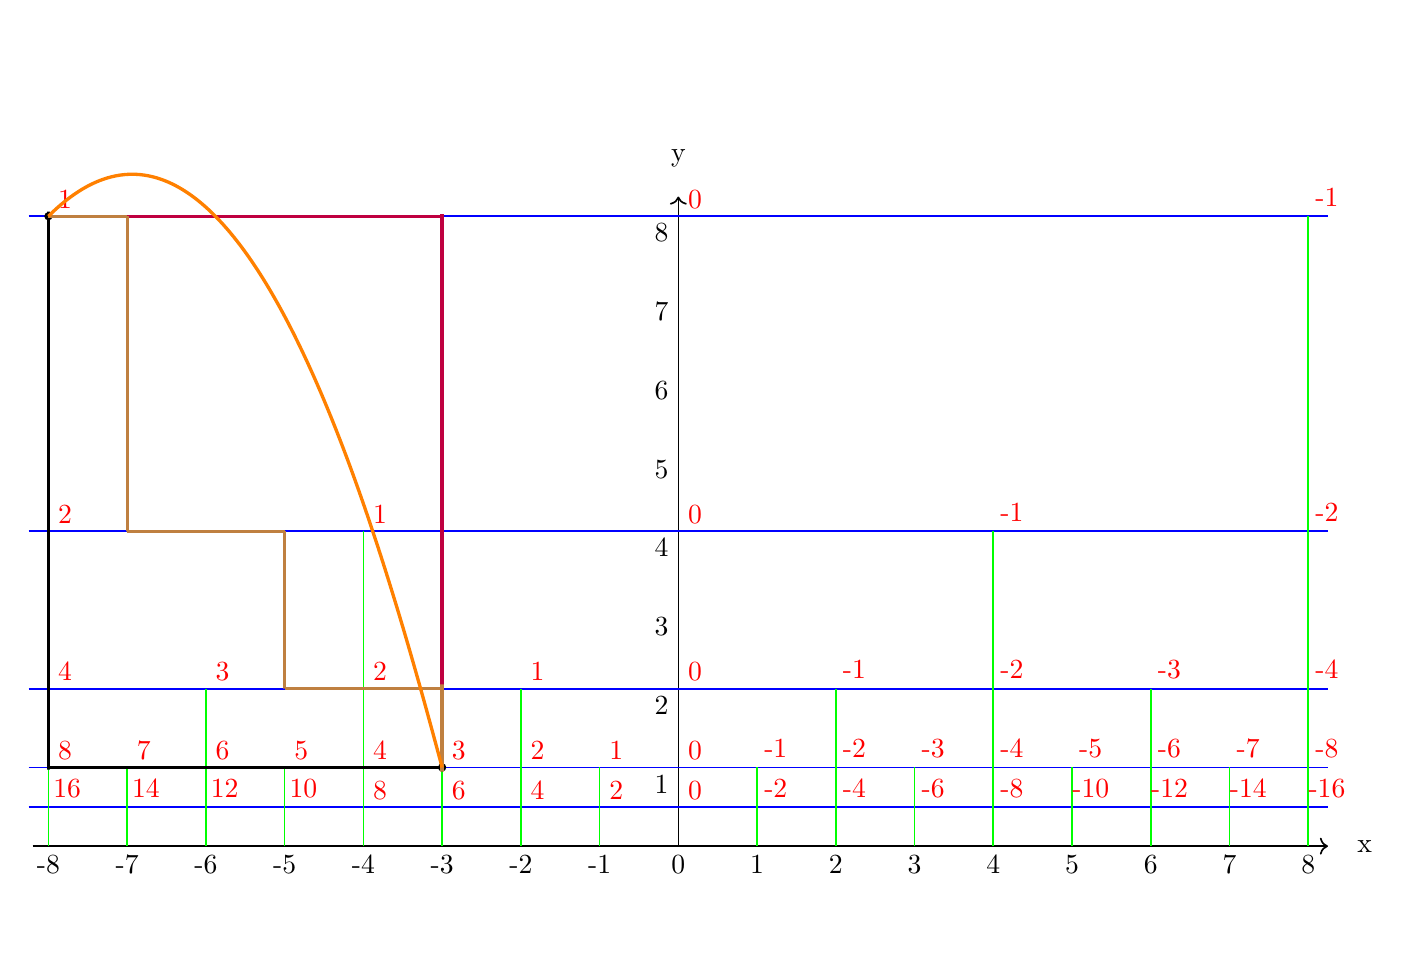
\begin{tikzpicture}
                \draw [black, line width=0.6pt, ->] (0,0) to[out=90,in=270] (0,8.25);
                \node [anchor=south] at (0,8.5) {y};
                \draw [black, line width=0.6pt, ->] (-8.2,0) to[out=0,in=180] (8.25,0);
                \node [anchor=west] at (8.5,0) {x};
                \foreach \x in {-8,-7,-6,-5,-4,-3,-2,-1,0,1,2,3,4,5,6,7,8}
                \node [anchor=north] at (\x,0) {\x};
                \foreach \y in {1,2,3,4,5,6,7,8}
                \node [anchor=45] at (0,\y) {\y};

                \draw [blue, line width=0.6pt] (-8.25,0.5) to[out=0,in=180] (8.25,0.5);
                \draw [blue, line width=0.6pt] (-8.25,1) to[out=0,in=180] (8.25,1);
                \draw [blue, line width=0.6pt] (-8.25,2) to[out=0,in=180] (8.25,2);
                \draw [blue, line width=0.6pt] (-8.25,4) to[out=0,in=180] (8.25,4);
                \draw [blue, line width=0.6pt] (-8.25,8) to[out=0,in=180] (8.25,8);

                \draw [green, line width=0.6pt] (-8,0) to[out=90,in=270] (-8,1);
                \draw [green, line width=0.6pt] (-7,0) to[out=90,in=270] (-7,1);
                \draw [green, line width=0.6pt] (-6,0) to[out=90,in=270] (-6,1);
                \draw [green, line width=0.6pt] (-5,0) to[out=90,in=270] (-5,1);
                \draw [green, line width=0.6pt] (-4,0) to[out=90,in=270] (-4,1);
                \draw [green, line width=0.6pt] (-3,0) to[out=90,in=270] (-3,1);
                \draw [green, line width=0.6pt] (-2,0) to[out=90,in=270] (-2,1);
                \draw [green, line width=0.6pt] (-1,0) to[out=90,in=270] (-1,1);
                \draw [green, line width=0.6pt] (1,0) to[out=90,in=270] (1,1);
                \draw [green, line width=0.6pt] (2,0) to[out=90,in=270] (2,1);
                \draw [green, line width=0.6pt] (3,0) to[out=90,in=270] (3,1);
                \draw [green, line width=0.6pt] (4,0) to[out=90,in=270] (4,1);
                \draw [green, line width=0.6pt] (5,0) to[out=90,in=270] (5,1);
                \draw [green, line width=0.6pt] (6,0) to[out=90,in=270] (6,1);
                \draw [green, line width=0.6pt] (7,0) to[out=90,in=270] (7,1);
                \draw [green, line width=0.6pt] (8,0) to[out=90,in=270] (8,1);

                \draw [green, line width=0.6pt] (-8,1) to[out=90,in=270] (-8,2);
                \draw [green, line width=0.6pt] (-6,1) to[out=90,in=270] (-6,2);
                \draw [green, line width=0.6pt] (-4,1) to[out=90,in=270] (-4,2);
                \draw [green, line width=0.6pt] (-2,1) to[out=90,in=270] (-2,2);
                \draw [green, line width=0.6pt] (2,1) to[out=90,in=270] (2,2);
                \draw [green, line width=0.6pt] (4,1) to[out=90,in=270] (4,2);
                \draw [green, line width=0.6pt] (6,1) to[out=90,in=270] (6,2);
                \draw [green, line width=0.6pt] (8,1) to[out=90,in=270] (8,2);

                \draw [green, line width=0.6pt] (-8,2) to[out=90,in=270] (-8,4);
                \draw [green, line width=0.6pt] (-4,2) to[out=90,in=270] (-4,4);
                \draw [green, line width=0.6pt] (4,2) to[out=90,in=270] (4,4);
                \draw [green, line width=0.6pt] (8,2) to[out=90,in=270] (8,4);

                \draw [green, line width=0.6pt] (-8,4) to[out=90,in=270] (-8,8);
                \draw [green, line width=0.6pt] (8,4) to[out=90,in=270] (8,8);

                \node [anchor=225, red] at (-8,0.5) {16};
                \node [anchor=225, red] at (-7,0.5) {14};
                \node [anchor=225, red] at (-6,0.5) {12};
                \node [anchor=225, red] at (-5,0.5) {10};
                \node [anchor=225, red] at (-4,0.5) {8};
                \node [anchor=225, red] at (-3,0.5) {6};
                \node [anchor=225, red] at (-2,0.5) {4};
                \node [anchor=225, red] at (-1,0.5) {2};
                \node [anchor=225, red] at (0,0.5) {0};
                \node [anchor=225, red] at (1,0.5) {-2};
                \node [anchor=225, red] at (2,0.5) {-4};
                \node [anchor=225, red] at (3,0.5) {-6};
                \node [anchor=225, red] at (4,0.5) {-8};
                \node [anchor=225, red] at (5,0.5) {-10};
                \node [anchor=225, red] at (6,0.5) {-12};
                \node [anchor=225, red] at (7,0.5) {-14};
                \node [anchor=225, red] at (8,0.5) {-16};

                \node [anchor=225, red] at (-8,1) {8};
                \node [anchor=225, red] at (-7,1) {7};
                \node [anchor=225, red] at (-6,1) {6};
                \node [anchor=225, red] at (-5,1) {5};
                \node [anchor=225, red] at (-4,1) {4};
                \node [anchor=225, red] at (-3,1) {3};
                \node [anchor=225, red] at (-2,1) {2};
                \node [anchor=225, red] at (-1,1) {1};
                \node [anchor=225, red] at (0,1) {0};
                \node [anchor=225, red] at (1,1) {-1};
                \node [anchor=225, red] at (2,1) {-2};
                \node [anchor=225, red] at (3,1) {-3};
                \node [anchor=225, red] at (4,1) {-4};
                \node [anchor=225, red] at (5,1) {-5};
                \node [anchor=225, red] at (6,1) {-6};
                \node [anchor=225, red] at (7,1) {-7};
                \node [anchor=225, red] at (8,1) {-8};

                \node [anchor=225, red] at (-8,2) {4};
                \node [anchor=225, red] at (-6,2) {3};
                \node [anchor=225, red] at (-4,2) {2};
                \node [anchor=225, red] at (-2,2) {1};
                \node [anchor=225, red] at (0,2) {0};
                \node [anchor=225, red] at (2,2) {-1};
                \node [anchor=225, red] at (4,2) {-2};
                \node [anchor=225, red] at (6,2) {-3};
                \node [anchor=225, red] at (8,2) {-4};

                \node [anchor=225, red] at (-8,4) {2};
                \node [anchor=225, red] at (-4,4) {1};
                \node [anchor=225, red] at (0,4) {0};
                \node [anchor=225, red] at (4,4) {-1};
                \node [anchor=225, red] at (8,4) {-2};

                \node [anchor=225, red] at (-8,8) {1};
                \node [anchor=225, red] at (0,8) {0};
                \node [anchor=225, red] at (8,8) {-1};

                \node[circle,fill=black,inner sep=1pt,minimum size=3pt] (a) at (-8,8) {};
                \node[circle,fill=black,inner sep=1pt,minimum size=3pt] (b) at (-3,1) {};

                \draw [black, line width=1.2pt] (-8,7.7) to[out=90,in=270] (-8,1.33);
                \draw [black, line width=1.2pt] (-8,1) to[out=0,in=180] (-3,1);

                \draw [purple, line width=1.2pt] (-8,8) to[out=0,in=180] (-3,8);
                \draw [purple, line width=1.2pt] (-3,7.67) to[out=90,in=270] (-3,1.33);

                \draw [brown, line width=1.2pt] (-8,8) to[out=0,in=180] (-7,8);
                \draw [brown, line width=1.2pt] (-7,7.8) to[out=90,in=270] (-7,4.2);
                \draw [brown, line width=1.2pt] (-7,4) to[out=0,in=180] (-5,4);
                \draw [brown, line width=1.2pt] (-5,3.9) to[out=90,in=270] (-5,2.1);
                \draw [brown, line width=1.2pt] (-5,2) to[out=0,in=180] (-3,2);
                \draw [brown, line width=1.2pt] (-3,2) to[out=90,in=270] (-3,1);

                \draw [orange, line width=1.2pt] (-8,8) to[out=45,in=105] (-3,1);

            \end{tikzpicture}
        }
        \label{fig:pathex1}
    \end{figure}
\end{frame}

\begin{frame}
    \frametitle{Arithmetic torsion at scale}
    \begin{columns}
        \begin{column}{0.5\textwidth}
            As the step size increases:

            For a single step:
            \begin{equation}
            (x + 1) \times 2 - (x \times 2 + 1) = 1
            \end{equation}

            For two steps:
            \begin{equation}
            (x + 2) \times 4 - (x \times 4 + 2) = 6
            \end{equation}

            For three steps, the pattern continues:
            \begin{equation}
            (x + 3) \times 8 - (x \times 8 + 3) = 21
            \end{equation}
        \end{column}
        \begin{column}{0.5\textwidth}
            \begin{center}
                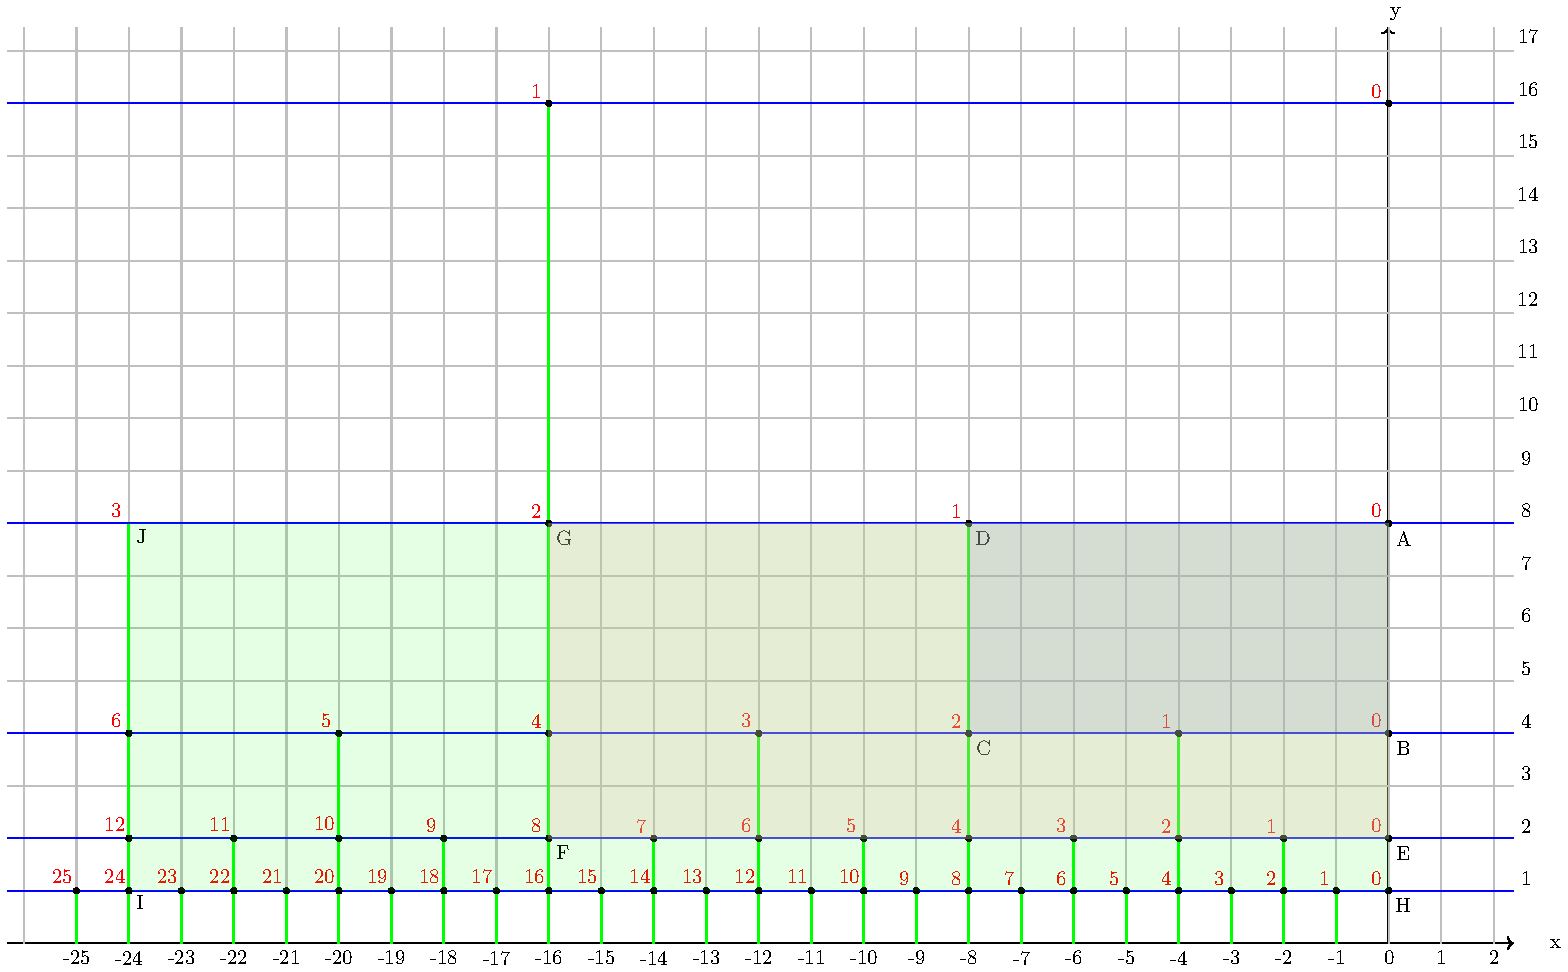
\includegraphics[width=1.0\textwidth]{../images/17-area-formula}
            \end{center}
        \end{column}
    \end{columns}
\end{frame}

\begin{frame}
    \frametitle{Eigenfunction of the Laplacian}
    In this setting, \(A = \frac{1}{\mu y}\) and \(B = \frac{1}{\lambda y}\):

    \[
        \Delta f = y^2 \left(\mu^2 \frac{\partial^2 f}{\partial x^2} + \lambda^2 \frac{\partial^2 f}{\partial y^2}\right)
    \]

    For \(f = -\frac{x}{y}\), it follows that

    \[
        \Delta f = - \frac{2 \lambda^2 x}{y} = 2 \lambda^2 f
    \]

    Therefore, \(f = -\frac{x}{y}\) is an eigenfunction of the Laplacian with eigenvalue \(2\lambda^2\).
\end{frame}

\begin{frame}
    \frametitle{When the Alexander polynomial meets the cyclotomic polynomial}
    \begin{itemize}
        \item The figure-eight knot $(4_1)$ has Alexander polynomial $\Delta_{4_1}(t)=t^2-3t+1$.
        \item An AEG path closes precisely when $\Delta_{4_1}(t)=0$.
        \item Cyclotomic polynomials appear in the global arithmetic torsion of the AEG path; for example, $$\tau(a) = \frac{-\Delta_{4_1}(a)(a^2-1)}{a^2}$$.
    \end{itemize}
    \vspace{0.2cm}
    \begin{columns}
        \begin{column}{0.48\textwidth}
            \begin{center}
                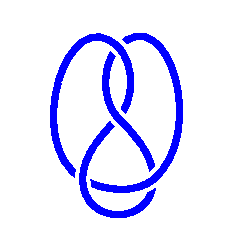
\includegraphics[width=0.4\textwidth]{../images/knot_4_1}

                {\small $4_1$ knot}
            \end{center}
        \end{column}
        \begin{column}{0.48\textwidth}
            \begin{center}
                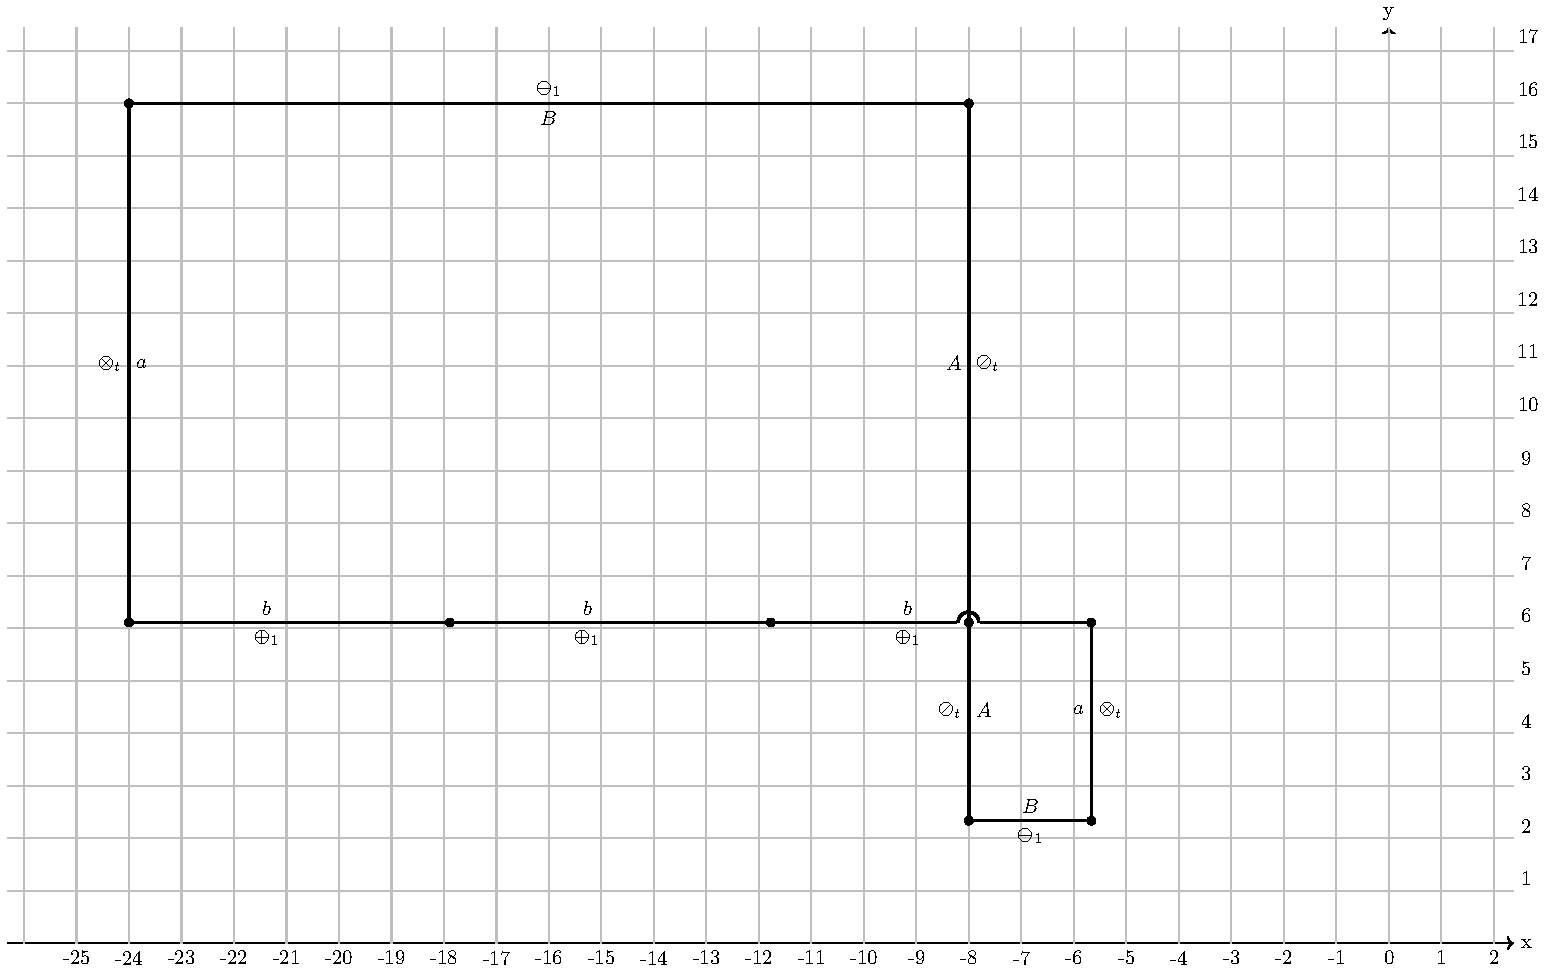
\includegraphics[width=0.6\textwidth]{../images/alexander_4_1}
                
                {\small Alexander-coded path}
            \end{center}
        \end{column}
    \end{columns}
\end{frame}

\begin{frame}
    \frametitle{Binary numeral as flow}
            Examples:
    \begin{center}
         $\left(\frac{3}{2}\right)_{10} = 1.1_{2},\ \left(\frac{7}{4}\right)_{10} = 1.11_{2},\ \left(\frac{21}{8}\right)_{10} = 10.101_{2}.$
        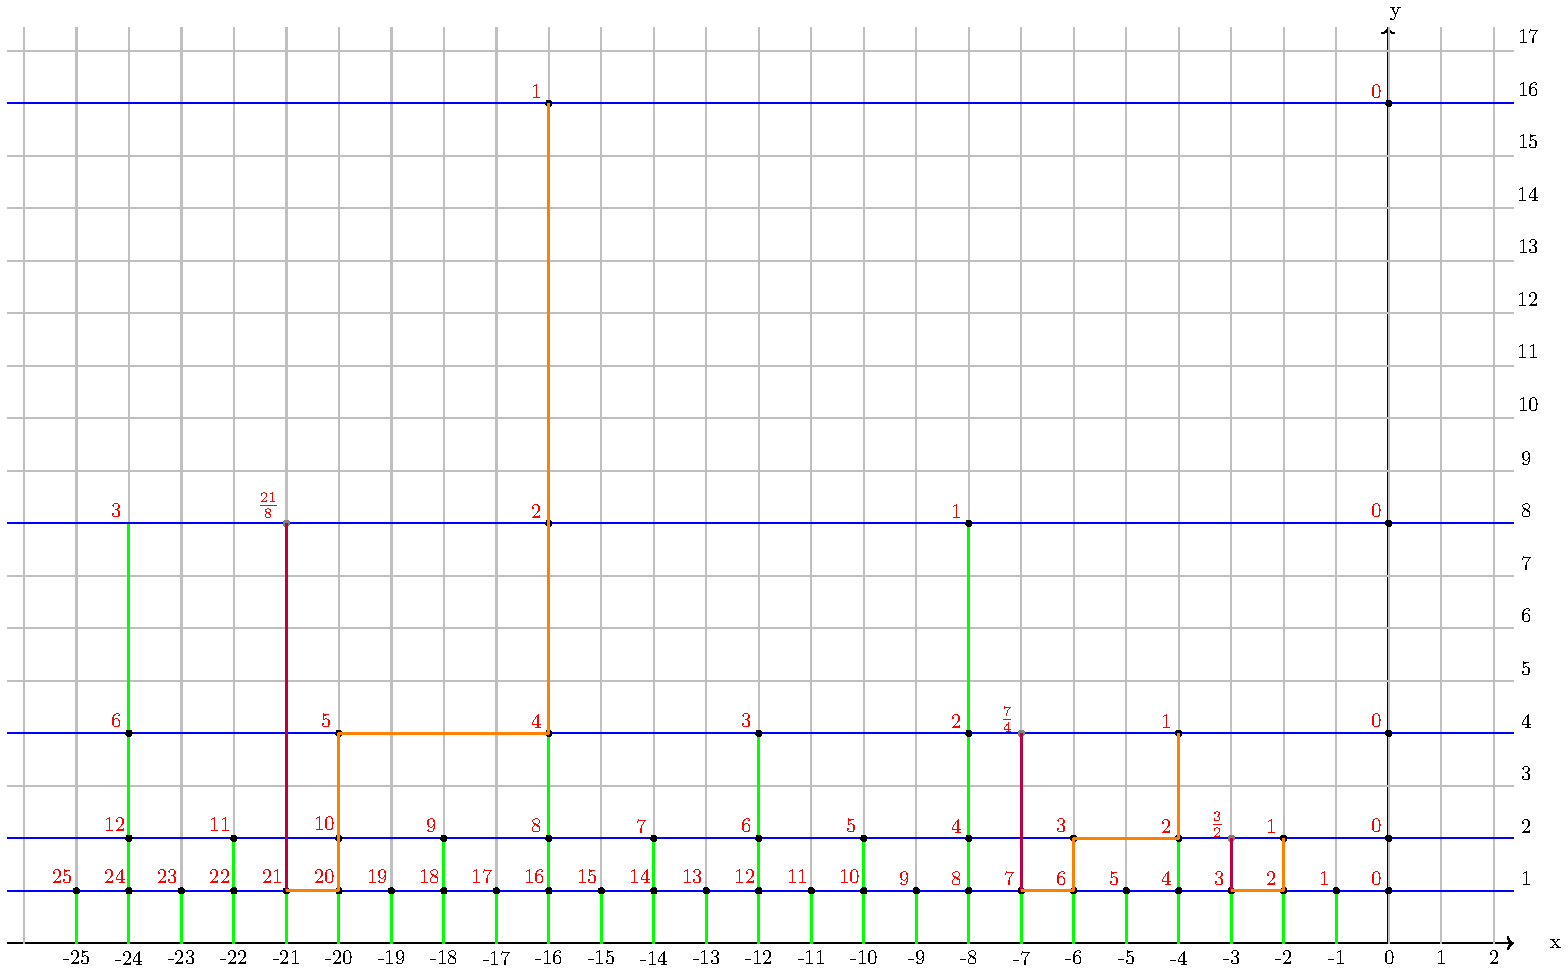
\includegraphics[width=0.7\textwidth]{../images/multiplication}
    \end{center}
\end{frame}

\begin{frame}
    \frametitle{Which complexity does volume measure?}
    It is well known that time and space complexity can trade off against one another.
    \begin{itemize}
        \item Time complexity: number of operations (steps)
        \item Space complexity: memory usage (intermediate results)
    \end{itemize}
    This trade-off suggests a common source of complexity. Which notion of complexity does geometric volume quantify?
\end{frame}

\begin{frame}
    \frametitle{Conclusion: richness from the unified perspective}
    We have shown that:
    \begin{itemize}
        \item Arithmetic expressions can be encoded as geometric flows in the hyperbolic model $\mathfrak{E}_1$; the assignment $a=-x/y$ links computation, geometry, and analysis via the flow equation.
        \item Non-commutativity manifests as arithmetic torsion that scales with step size and organizes paths; analytic structure appears through Laplacian eigenfunctions.
        \item Algebraic invariants such as Alexander and cyclotomic polynomials govern path closure and global torsion, revealing a deep interface between topology and arithmetic.
    \end{itemize}
\end{frame}

%%%%%%%%%%%%%%%%%%%%%%%%%%%%%%%%%%%%%%%%%%%%%%%%%%%%%%%%%%%%%%%%%%%%%%%%%%%%%%%
% Possibility 3: A Neo-Calculus?
%%%%%%%%%%%%%%%%%%%%%%%%%%%%%%%%%%%%%%%%%%%%%%%%%%%%%%%%%%%%%%%%%%%%%%%%%%%%%%%

\section{Malachite: The green stone of renewal}

\begin{frame}
    \frametitle{Malachite: The green stone of renewal}
    \begin{center}
        \Large
        \textbf{A Neo-Calculus?}\newline\newline
        \emph{Can we develop a new calculus that naturally handles mixed operations?}
    \end{center}
\end{frame}

\begin{frame}
    \frametitle{How to describe a change over time?}
    \begin{columns}
        \begin{column}{0.7\textwidth}
            Two complementary ways to describe a small change over time:
            \begin{itemize}
                \item by quantity: add a near-zero amount
                \item by ratio: multiply by a near-unit factor
            \end{itemize}
            Traditional calculus is based on the first method; the Riemann integral is additive.
            The functions $\exp$ and $\log$ convert between these two viewpoints.
        \end{column}
        \begin{column}{0.3\textwidth}
            \begin{figure}[ht]\centering
            \resizebox{1.0\textwidth}{!}{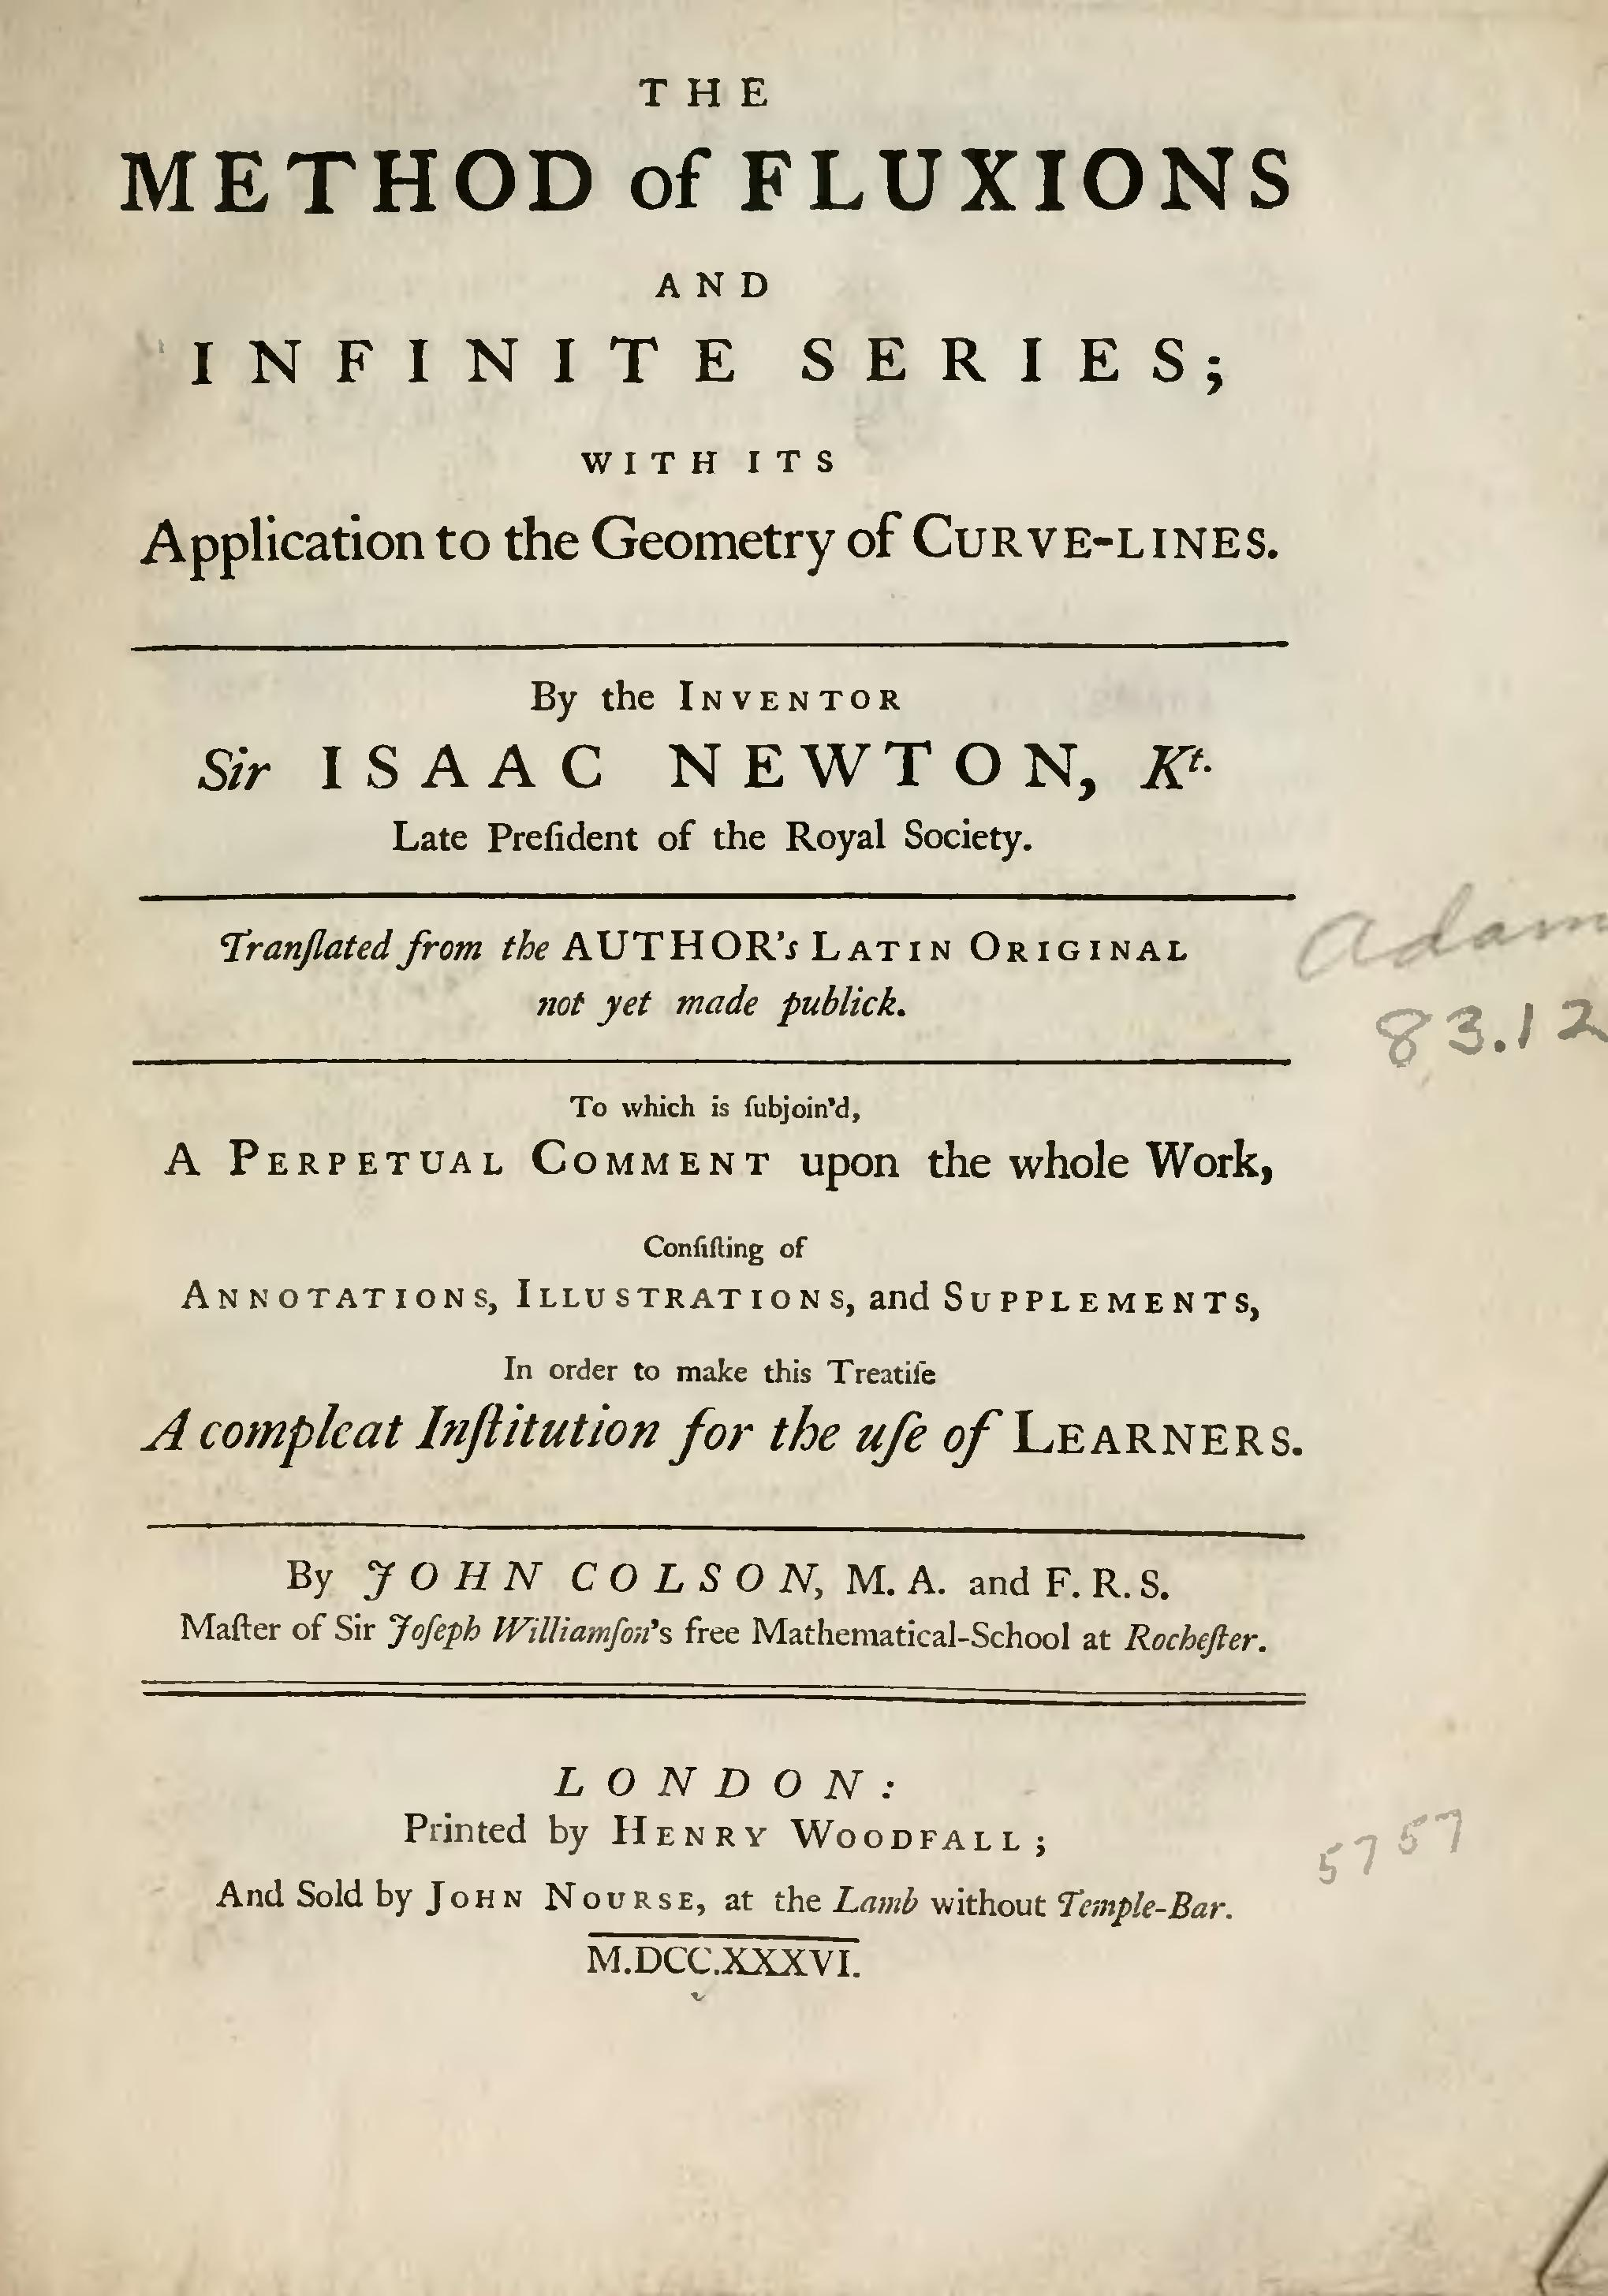
\includegraphics{../images/fluxions}}
            \caption{Method of Fluxions}
            \end{figure}
        \end{column}
    \end{columns}
\end{frame}

\begin{frame}
    \frametitle{Product integration}
    \begin{columns}
            \begin{column}{0.3\textwidth}
                \begin{figure}[ht]\centering
                \resizebox{1.0\textwidth}{!}{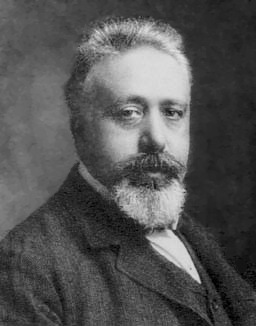
\includegraphics{../images/vito_volterra}}
                \caption{Vito Volterra}
                \end{figure}
            \end{column}
            \begin{column}{0.7\textwidth}
            Matrix-valued non-commutative differentiation and integration, left and right
            \begin{itemize}
                \item $\frac{d}{dx} A(x) = \lim_{\Delta x \to 0} \frac{A(x + \Delta x) A^{-1}(x) - I}{\Delta x}$
                \item $A(x) \frac{d}{dx} = \lim_{\Delta x \to 0} \frac{A^{-1}(x) A(x + \Delta x) - I}{\Delta x}$
                \item $\prod_{a}^{b} (I + A(x) dx) = \lim_{\nu(P) \to 0} \prod_{i=m}^{1}(I + A(\xi_i))$
                \item $(I + A(x) dx) \prod_{a}^{b}  = \lim_{\nu(P) \to 0} \prod_{i=1}^{m}(I + A(\xi_i))$
            \end{itemize}
            An identity connects product integration with standard additive integration:
            \[
              \prod_a^b (I + A(x)\,dx)
              = I + \int_a^b A(x)\,dx + \int_a^b \int_a^x A(x)A(y)\,dy\,dx + \cdots
            \]
            \end{column}
    \end{columns}
\end{frame}

\begin{frame}
    \frametitle{How about mixing up additive and multiplicative steps?}
    Additive calculus provides a closed algebra of polynomials under differential and integral operators.
    \begin{itemize}
        \item $\frac{d}{dx} p(x) = q(x)$
        \item $\int p(x)\,dx = q(x) + C$
    \end{itemize}
    This underlies power series, Laurent series, and approximation theory.
    \newline\newline
    Problem: How do we mix additive and multiplicative steps in a single process?
    \newline\newline
    Directions:
    \begin{itemize}
        \item We need to handle functions beyond constants in arithmetic expressions.
        \item We need to expand polynomials into another closed set under differential and integral operators.
    \end{itemize}
\end{frame}

\begin{frame}
    \frametitle{A contact structure}
    Consider $(u,v,a)\in\mathbb{R}^3$ with constants $\mu,\lambda$.
    \[
      \omega := \mu\,du + \lambda a\,dv,\qquad \alpha := da - \omega
    \]
    Key properties:
    \begin{itemize}
      \item Contact:
      \[
        d\omega=\lambda\,da\wedge dv,\quad d\alpha=-d\omega,\quad
        \alpha\wedge d\alpha=\mu\lambda\,du\wedge da\wedge dv\neq 0
      \]
      so $\alpha$ is a contact form when $\mu\lambda\neq 0$.
      \item Reeb field and distribution:
      \[
        R=-(1/\mu)\,\partial_u,\qquad \mathcal{H}:=\ker\alpha
      \]
      \item Horizontal lifts (basis of $\mathcal{H}$):
      \[
        D_u:=\partial_u+\mu\,\partial_a,\qquad
        D_v:=\partial_v+\lambda a\,\partial_a,\qquad \alpha(D_u)=\alpha(D_v)=0
      \]
      \item Natural units: with $\tilde u=\mu u,\ \tilde v=\lambda v$,
      \[
        \alpha=da-d\tilde u-a\,d\tilde v
      \]
    \end{itemize}
\end{frame}

\begin{frame}
    \frametitle{Calculus over the contact structure: I}
    The expression differential $\delta$ is defined by
    \[
      \delta a=\omega,\qquad \delta u=du,\qquad \delta v=dv,
    \]
    and for any $F(u,v,a)$
    \[
      \delta F = dF - (\partial_a F)\,\alpha
      = (D_uF)\,du + (D_vF)\,dv,
    \]
    where
    \[
      D_uF=F_u+\mu F_a,\qquad D_vF=F_v+\lambda a F_a,\qquad
      D_\theta=\cos\theta\,D_u+\sin\theta\,D_v.
    \]
    Chain rules:
    \[
      \delta\Phi(a)=\Phi'(a)\,\omega,\qquad
      \delta F(E_1,E_2)=\partial_1F\,\delta E_1+\partial_2F\,\delta E_2.
    \]
\end{frame}

\begin{frame}
    \frametitle{Calculus over the contact structure: II}
    Curvature and non-commutativity:
    \[
      [D_u,D_v]=\mu\lambda\,\partial_a,\qquad
      \delta^2F=\mu\lambda(\partial_a F)\,du\wedge dv,\qquad
      \delta^2 a=\mu\lambda\,du\wedge dv.
    \]
    Compatibility and circulation:
    \[
      (d\omega)^*\big|_{\alpha=0}=\mu\lambda\,du\wedge dv,\qquad
      \oint_{\partial\Sigma}\omega=\iint_\Sigma d\omega=\mu\lambda\iint_\Sigma du\wedge dv.
    \]
    Quick rules:
    \[
      \delta(a^n)=n a^{n-1}\omega,\quad
      \delta(\ln a)=\tfrac{\omega}{a},\quad
      \delta(e^a)=e^a\omega,\quad
      \delta(\sin a)=\cos a\,\omega,\quad
      \delta(\cos a)=-\sin a\,\omega.
    \]
    Rectification and flow:
    \[
      y=\arcsin\!\left(\tfrac{\lambda a}{\mu}\right),\quad \|\nabla y\|=\lambda,\quad
      \frac{da}{ds}=D_\theta a=\mu\cos\theta+\lambda a\sin\theta.
    \]
\end{frame}

\begin{frame}
  \frametitle{Extending polynomials: the affine–Appell basis}
  Natural units: $\tilde u=\mu u,\ \tilde v=\lambda v$. Define scaled powers
  \[
    B_n(a,v):=e^{-n\tilde v}a^n\quad(n\in\mathbb{N}).
  \]
  Let
  \[
    \mathcal{B}:=\Big\{\sum_{n=0}^N P_n(u,v,e^{\tilde v})\,B_n(a,v)\ \text{(finite)}\Big\}.
  \]
  \textbf{Closure Theorem.} $\mathcal{B}$ is closed under the mixed calculus generated by
  \[
    D_u=\partial_u+\mu\,\partial_a,\qquad D_v=\partial_v+\lambda a\,\partial_a.
  \]
  Rules:
  \[
    D_u(PB_n)=(\partial_u P)B_n+\mu n\,e^{-\tilde v}P\,B_{n-1},\quad
    D_v(PB_n)=(\partial_v P)B_n.
  \]
\end{frame}

\begin{frame}
  \frametitle{Antiderivatives and a finite upward sweep}
  If $P$ is independent of $u$,
  \[
    D_u^{-1}\!\big(P(v,e^{\tilde v})\,B_n\big)=\frac{e^{\tilde v}P(v,e^{\tilde v})}{\mu(n+1)}\,B_{n+1}.
  \]
  In general, define $Q^{(0)}_n=\dfrac{e^{\tilde v}}{\mu(n+1)}P_n$ and set $G^{(0)}=\sum_n Q^{(0)}_nB_{n+1}$.
  Then $F-\!D_uG^{(0)}=-\sum_n(\partial_uQ^{(0)}_n)B_{n+1}$. Repeat for finitely many steps.
  \vspace{0.6em}

  \textbf{Example.} For $F=a^3e^{\lambda v}=e^{4\tilde v}B_3$,
  \[
    D_u^{-1}F=\frac{e^{\tilde v}}{4\mu}B_4=\frac{e^{\lambda v}}{4\mu}a^4,\quad
    D_u\!\left(\frac{e^{\lambda v}}{4\mu}a^4\right)=a^3e^{\lambda v}.
  \]
\end{frame}

\begin{frame}
    \frametitle{Conclusion: a new calculus for mixed operations}
    We have shown that:
    \begin{itemize}
        \item Mixed additive/multiplicative change admits a contact geometry on $(u,v,a)$ with $\alpha=da-\omega$, $\omega=\mu\,du+\lambda a\,dv$; $\mathcal{H}=\ker\alpha$ has basis $\{D_u,D_v\}$ and $\alpha$ is contact for $\mu\lambda\neq 0$.
        \item The expression differential $\delta$ projects $d$ to $\ker\alpha$: $\delta F=dF-(\partial_aF)\alpha$, with chain rules and directional synthesis via $D_\theta$.
        \item Non-commutativity/curvature are encoded by $[D_u,D_v]=\mu\lambda\,\partial_a$ and $\delta^2F=\mu\lambda(\partial_aF)\,du\wedge dv$; circulation-area and de Rham compatibility hold.
        \item Legendrian flow obeys $\frac{da}{ds}=\mu\cos\theta+\lambda a\sin\theta$; rectification $y=\arcsin(\lambda a/\mu)$ yields $\|\nabla y\|=\lambda$ and stabilizes numerics; natural units $(\tilde u,\tilde v)$ simplify formulas.
        \item An affine–Appell basis $B_n(a,v)=e^{-n\tilde v}a^n$ is closed under $D_u,D_v$, enabling explicit differentiation/integration and constructive antiderivatives for mixed expressions.
    \end{itemize}
\end{frame}

%%%%%%%%%%%%%%%%%%%%%%%%%%%%%%%%%%%%%%%%%%%%%%%%%%%%%%%%%%%%%%%%%%%%%%%%%%%%%%%
% Possibility 4: A New Atlas for Complex Analysis?
%%%%%%%%%%%%%%%%%%%%%%%%%%%%%%%%%%%%%%%%%%%%%%%%%%%%%%%%%%%%%%%%%%%%%%%%%%%%%%%

\section{Quartz: The white stone of clarity}

\begin{frame}
    \frametitle{Quartz: The white stone of clarity}
    \begin{center}
        \Large
        \textbf{A New Atlas for Complex Analysis?}
        \newline\newline
        \emph{Is complex analysis a special case of a more general theory?}
    \end{center}
\end{frame}

\begin{frame}
    \frametitle{Why are complex numbers necessary here?}
    This stems from the fact that multiplication by $-1$ is involutive, i.e., $(-1)^2=1$.
    We therefore need an infinitesimal generator that connects $-1$ and $1$ continuously.

    \vspace{0.2cm}

    \begin{figure}[ht]\centering
    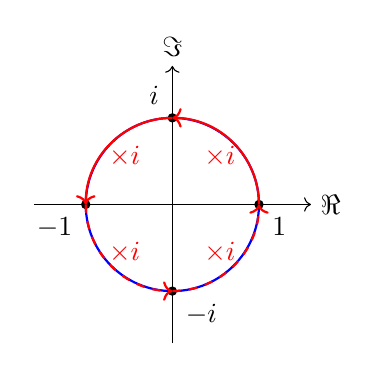
\begin{tikzpicture}[scale=1.1]
      % axes
      \draw[->] (-1.6,0) -- (1.6,0) node[right] {$\Re$};
      \draw[->] (0,-1.6) -- (0,1.6) node[above] {$\Im$};
      % unit circle
      \draw[thick, blue] (0,0) circle (1);
      % points
      \node[fill,circle,inner sep=1.2pt, label={below right:$1$}] (one) at (1,0) {};
      \node[fill,circle,inner sep=1.2pt, label={below left:$-1$}] (minusone) at (-1,0) {};
      \node[fill,circle,inner sep=1.2pt, label={above left:$i$}] (ii) at (0,1) {};
      \node[fill,circle,inner sep=1.2pt, label={below right:$-i$}] (minusi) at (0,-1) {};
      % arcs: multiplication by i (90-degree rotations)
      \draw[->, red, thick] (1,0) arc[start angle=0, end angle=90, radius=1];
      \draw[->, red, thick] (0,1) arc[start angle=90, end angle=180, radius=1];
      \draw[->, red, thick, dashed] (-1,0) arc[start angle=180, end angle=270, radius=1];
      \draw[->, red, thick, dashed] (0,-1) arc[start angle=270, end angle=360, radius=1];
      % labels on arcs
      \node[red] at (0.55,0.55) {$\times i$};
      \node[red] at (-0.55,0.55) {$\times i$};
      \node[red] at (-0.55,-0.55) {$\times i$};
      \node[red] at (0.55,-0.55) {$\times i$};
    \end{tikzpicture}
    \caption{$i$ as a generator: multiplication by $i$ rotates by $90^\circ$, so $1 \xrightarrow{\times i} i \xrightarrow{\times i} -1$.}
    \end{figure}
\end{frame}

\begin{frame}
  \frametitle{Setup (over $\mathbb C$): contact structure and affine--Appell chart}
  \textbf{Complexification rule.} Coordinates $(u,v)\in\mathbb R^2$; values and parameters
  $a,\mu,\lambda\in\mathbb C$. All operators act $\mathbb C$-linearly.

  \vspace{0.4em}
  \textbf{Contact data and horizontal fields}
  \[
    \omega:=\mu\,du+\lambda a\,dv,\qquad
    \alpha:=da-\omega,
  \]
  \[
    D_u:=\partial_u+\mu\,\partial_a,\qquad
    D_v:=\partial_v+\lambda a\,\partial_a,\qquad
    \delta F=(D_uF)\,du+(D_vF)\,dv.
  \]
  \vspace{0.4em}

  \textbf{Natural units and affine--Appell coordinate}
  \[
    \tilde u:=\mu u,\quad \tilde v:=\lambda v,\qquad
    s:=a\,e^{-\tilde v}\ \Rightarrow\ D_v s=0,\ D_u s=\mu\,e^{-\tilde v}.
  \]
  We write $B_n:=s^n\ (n\in\mathbb N)$ and use an EL-closed coefficient ring
  $\mathcal R_{\mathrm{EL}}$ generated by $u,v,e^{\pm\tilde v}$ and closed under
  $+,\times,\partial_u,\partial_v,\exp,\log$ (where defined).
\end{frame}

\begin{frame}
  \frametitle{Definition and intuition: AEG--Cauchy--Riemann over $\mathbb C$}
  \textbf{Arithmetic-holomorphic (over $\mathbb C$).} For $h=f+ig$ with $f,g:\ (u,v,a)\mapsto\mathbb R$,
  define
  \[
    \bar{D}:=\tfrac12\,(D_u+iD_v),\qquad \text{AEG-holomorphic} \iff \bar{D}h=0.
  \]
  Equivalently, the \textbf{AEG--CR equations}
  \[
    D_u f=D_v g,\qquad D_v f=-D_u g. \tag{16}
  \]

  \textbf{Geometric consequences.}
  \begin{itemize}
    \item \emph{Conformality and equal norms}:
      $(D_uf,D_ug)\perp(D_vf,D_vg)$ and
      $(D_uf)^2+(D_ug)^2=(D_vf)^2+(D_vg)^2$.
    \item \emph{Classical limit}: if $f,g$ are independent of $a$, then
      $D_u=\partial_u,\ D_v=\partial_v$, yielding the usual CR equations on $(u,v)$.
    \item \emph{Rigidity}: if $f=f(a)$ and $g=g(a)$, the only solutions are constants.
  \end{itemize}
\end{frame}

\begin{frame}
  \frametitle{AEG--Weierstrass expansion in the affine--Appell chart}
  \textbf{Theorem (local expansion and uniqueness).}
  Let $h=f+ig$ be $C^1$ on a neighborhood and satisfy $\bar{D}h=0$.
  Then there exist unique coefficients $A_n(u,v)\in\mathcal R_{\mathrm{EL}}$ (real-analytic in $(u,v)$)
  such that
  \[
    h(u,v,a)=\sum_{n\ge0} A_n(u,v)\,s^n,\qquad s=a\,e^{-\tilde v}.
  \]
  The coefficients obey the triangular recursion
  \[
    \frac{\mu}{2}\,e^{-\tilde v}\,(m+1)\,A_{m+1}(u,v)+\partial_{\bar\zeta}A_m(u,v)=0,
    \quad \partial_{\bar\zeta}:=\tfrac12(\partial_u+i\partial_v).
  \]
  Conversely, any convergent series with this recursion solves $\bar{D}h=0$.

  \textbf{Meromorphic extension.} Allowing a finite principal part
  $h=\sum_{n\ge N}A_n s^n$ ($N\in\mathbb Z$) yields AEG–meromorphic functions
  (poles at $s=0$).
\end{frame}

\begin{frame}
  \frametitle{Symbolic calculus and closure (computable rules)}
  For $F=\sum_{n\ge0}A_n s^n$:
  \[
    D_u F=\sum (\partial_u A_n)\,s^n+\mu e^{-\tilde v}\sum_{n\ge1} nA_n\,s^{n-1},\qquad
    D_v F=\sum (\partial_v A_n)\,s^n.
  \]
  \textbf{Indefinite integration along $u$.} Find $G=\sum B_n s^n$ with $D_uG=F$:
  \[
    B_0\ \text{free},\qquad
    B_{k+1}=\frac{A_k-\partial_u B_k}{\mu e^{-\tilde v}(k+1)}\quad(k\ge0).
  \]

  \textbf{Algebraic closure.}
  \begin{itemize}
    \item Closed under addition and the “AEG complex product”
      $(f,g)\odot(\tilde f,\tilde g)=(f\tilde f-g\tilde g,\ f\tilde g+\tilde f g)$.
    \item Composition with a classical holomorphic function of $\zeta=u+iv$ preserves AEG-holomorphicity.
    \item Laurent series in $s$ implement the AEG–meromorphic class (residues at $s=0$).
  \end{itemize}
\end{frame}

\begin{frame}
  \frametitle{Conformality, curvature density, and fiberwise complex analysis}
  Write $F=(f,g)$ and $|F'|^2:=(D_uf)^2+(D_ug)^2=(D_vf)^2+(D_vg)^2$. Then
  \[
    d\omega=\frac{\mu\lambda}{|F'|^2}\,df\wedge dg. \tag{17}
  \]
  The area density rescales by the Jacobian $|F'|^{-2}$, while the total integral
  $\int d\omega$ is invariant (expression-conformal coordinates).

  \vspace{0.5em}
  \textbf{Fiberwise complex analysis in $s$.}
  Fix $(u,v)$; then $s\in\mathbb C$ and $h(\,\cdot\,)=\sum A_n s^n$ is holomorphic in $s$.
  Hence the classical Cauchy machinery applies fiberwise:
  \[
    h(s_0)=\frac{1}{2\pi i}\oint_{\gamma}\frac{h(s)}{s-s_0}\,ds,\qquad
    \oint_{\gamma} h(s)\,ds=2\pi i\cdot A_{-1}(u,v),
  \]
  for any loop $\gamma$ encircling $s_0$ (or $0$ for the residue statement).
\end{frame}

\begin{frame}
  \frametitle{Constructors and examples over $\mathbb C$}
  \textbf{Constructor (seed $\Rightarrow$ AEG-holomorphic).}
  Pick any real-analytic seed $A_0(u,v)$; define recursively
  \[
    A_{m+1}(u,v)=-\,\frac{2\,e^{\tilde v}}{\mu\,(m+1)}\,\partial_{\bar\zeta}A_m(u,v),
    \qquad m\ge0,
  \]
  and set $h=\sum_{n\ge0}A_n s^n$ with $s=a\,e^{-\tilde v}$. Then $\bar{D}h=0$.
  If $A_0$ is classical holomorphic in $\zeta$, all higher $A_{n\ge1}$ vanish (classical limit).

  \vspace{0.5em}
  \textbf{Explicit nontrivial example.}
  Take $A_0(\zeta,\bar\zeta)=\bar\zeta$; then
  \[
    A_1=-\tfrac{2}{\mu}e^{\tilde v},\quad
    A_2=\tfrac{i\lambda}{\mu^2}e^{2\tilde v},\quad
    A_3=\tfrac{2\lambda^2}{3\mu^3}e^{3\tilde v},\ \ldots
  \]
  so
  \[
    h(u,v,a)=\bar\zeta-\frac{2}{\mu}\,a+\frac{i\lambda}{\mu^2}\,a^2+\frac{2\lambda^2}{3\mu^3}\,a^3+\cdots
  \]
  is AEG-holomorphic (convergent in a neighborhood controlled by $|a|$ and the majorant of $A_0$).
\end{frame}

\begin{frame}
    \frametitle{Conclusion: A new context for holomorphic and analytic functions}
    We have shown that:
    \begin{itemize}
        \item AEG–Cauchy–Riemann: $\bar D=\tfrac12(D_u+iD_v)$, with $\bar D h=0$ defining arithmetic holomorphicity; conformality and the classical limit are recovered, while rigidity appears for functions depending only on $a$.
        \item AEG–Weierstrass expansion: any local AEG–holomorphic $h$ admits $h=\sum_{n\ge0}A_n(u,v)\,s^n$ with triangular recursion; Laurent series in $s$ yield meromorphic extensions.
        \item Computation rules: explicit formulas for $D_u, D_v$ on series and a constructive scheme for indefinite integration along $u$; closure under the AEG complex product and composition with classical holomorphic maps in $\zeta=u+iv$.
        \item Geometry and analysis align: $d\omega=\frac{\mu\lambda}{|F'|^2}df\wedge dg$ encodes conformal area density; fiberwise in $s$, classical Cauchy integral and residue calculus apply.
    \end{itemize}
\end{frame}

%%%%%%%%%%%%%%%%%%%%%%%%%%%%%%%%%%%%%%%%%%%%%%%%%%%%%%%%%%%%%%%%%%%%%%%%%%%%%%%
% Possibility 5: A Key to the Non-linear Maze?
%%%%%%%%%%%%%%%%%%%%%%%%%%%%%%%%%%%%%%%%%%%%%%%%%%%%%%%%%%%%%%%%%%%%%%%%%%%%%%%

\section{Obsidian: The black stone of depth}

\begin{frame}
    \frametitle{Obsidian: The black stone of depth}
    \begin{center}
        \Large
        \textbf{A Key to the Nonlinear Maze?}
        \newline\newline
        \emph{Can AEG help us navigate the complexities of nonlinear systems?}
    \end{center}
\end{frame}

\begin{frame}
    \frametitle{Why is this possible?}
    \begin{itemize}
        \item The multiplicative dimension of AEG inherently encodes nonlinearity.
        \item The non-commutativity of operations is native to the AEG framework.
        \item A spatiotemporal view of complexity clarifies slow and fast variables in a synergetics setting.
    \end{itemize}
    In what follows, we show that AEG's Accumulative Commutative Space (ACS) functions as a minimalist RG flow.
\end{frame}

\begin{frame}
    \frametitle{ACS and RG: commutative coordinates and scale}
    \begin{itemize}
        \item Accumulative Commutative Space (ACS) assigns to any arithmetic path $\gamma$ the coordinates
        \[
            A_\gamma = \sum_k \mu_k,\qquad M_\gamma = \sum_k \lambda_k,
        \]
        where $\mu_k$ (additive) and $\lambda_k$ (log-multiplicative) are the operation parameters along $\gamma$.
        \item Interpretation:
        \begin{itemize}
            \item $A$ captures the \emph{net additive load} accumulated by the computation.
            \item $M$ encodes the \emph{evolutionary scale} (log-scale) accumulated by multiplicative steps.
        \end{itemize}
        \item Minimal RG perspective: varying $M$ probes effective dynamics (driven by addition and local flows) at different scales. ACS provides a commutative plane to compare paths across scales.
    \end{itemize}
\end{frame}

\begin{frame}
    \frametitle{AEG flow as a beta-function analog}
    \begin{itemize}
        \item Core flow equation for the assignment $a$ along direction $\theta$:
        \[
            \frac{da}{ds} = \mu \cos\theta + \lambda a \sin\theta,
        \]
        and a coordinate-independent magnitude
        \[
            \|\nabla a\| = \sqrt{\mu^2 + a^2\lambda^2}.
        \]
        \item RG analogy:
        \begin{itemize}
            \item The $\mu$ term contributes a scale-independent drive; the $\lambda a$ term contributes a \emph{scale-dependent} drive.
            \item Changing $M$ (accumulated $\lambda$) alters the relative influence of the multiplicative term, akin to scale-dependent couplings in RG.
        \end{itemize}
        \item Dual timescales: addition $\Rightarrow$ dynamical time; multiplication $\Rightarrow$ evolutionary time/scale. ACS tracks evolutionary time directly via $M$.
    \end{itemize}
\end{frame}

\begin{frame}
    \frametitle{Arithmetic torsion: scale-weighted invariant in ACS}
    \begin{itemize}
        \item Global arithmetic torsion for a surface $\Sigma_\gamma$ bounded by path $\gamma$:
        \[
            \tau(\gamma) = \iint_{\Sigma_\gamma} e^{M}\, dA \wedge dM.
        \]
        \item The factor $e^M$ \emph{weights} contributions by scale, embedding RG-like reweighting directly into the geometric invariant.
        \item Implications:
        \begin{itemize}
            \item Fixed points and phases leave characteristic signatures in ACS: e.g., $M\rightarrow -\infty$ (vanishing scale), $M=0$ (unit scale).
            \item Comparing paths at different scales becomes a surface integral in $(A,M)$ with explicit scale dependence.
        \end{itemize}
        \item This yields a minimalist renormalization lens: effective additive dynamics at evolutionary time $M$ are observed via ACS projections and torsion.
    \end{itemize}
\end{frame}

\begin{frame}
    \frametitle{Example I: Percolation RG ($R(p) = 3p^2 - 2p^3$)}
    \begin{itemize}
        \item Polynomial form $R(p)=Yp^N+Xp^{N-1}$ with $(X,Y,N)=(3,-2,3)$.
        \item ACS coordinates (canonical AEG path):
        \[
            A_R = X+Y = 1,\qquad M_R(p) = (N-1)\ln p = 2\ln p.
        \]
        \item Fixed points in ACS:
        \[
            p^*=0:\ (A=1,\ M\to -\infty),\quad
            p^*=\tfrac12:\ (A=1,\ M=-2\ln 2),
        \]
        \[
            p^*=1:\ (A=1,\ M=0).
        \]
        \item A torsion instance (path-dependent) $\mathcal{T}_R(p) = -\ln p\,(8p^{-1}+3)$ illustrates finite, nonzero torsion at the critical point and vanishing torsion at $p=1$.
    \end{itemize}
\end{frame}

\begin{frame}
    \frametitle{Example II: Logistic map ($R(x)=rx(1-x)$, $r=3.2$)}
    \begin{itemize}
        \item $R(x)=(-r)x^2+(r)x$ with $N=2$, coefficients $(c_2,c_1,c_0)=(-r,r,0)$.
        \item ACS coordinates (Horner path):
        \[
            A_R(r)=r,\qquad M_R(x)=2\ln x.
        \]
        \item Stable 2-cycle at $r=3.2$: $x_a\approx 0.513045$, $x_b\approx 0.799455$.
        \[
            M_R(x_a)\approx -1.3348,\quad M_R(x_b)\approx -0.4476.
        \]
        \item Second iterate $R^{(2)}$: $A_{R^{(2)}}=r^3=32.768$, $M_{R^{(2)}}(x)=4\ln x$. The points $x_a,x_b$ are fixed points of $R^{(2)}$, reflecting a deeper scale $M$.
    \end{itemize}
\end{frame}

\begin{frame}
    \frametitle{Takeaways: ACS as a minimalist RG flow}
    \begin{itemize}
        \item ACS provides $(A,M)$ coordinates that separate dynamical content (addition) from evolutionary scale (multiplication).
        \item The AEG flow encodes scale dependence directly via $\lambda a$, with $M$ acting as evolutionary time; varying $M$ reveals effective behavior at different scales.
        \item Arithmetic torsion integrates scale ($e^M$) into a geometric invariant, yielding phase-sensitive signatures and principled path comparisons.
        \item Across examples (percolation, logistic), fixed points and cycles appear as specific loci in ACS; $M$ quantifies scale while $A$ captures net additive load.
    \end{itemize}
\end{frame}



%%%%%%%%%%%%%%%%%%%%%%%%%%%%%%%%%%%%%%%%%%%%%%%%%%%%%%%%%%%%%%%%%%%%%%%%%%%%%%%
% Final Thoughts
%%%%%%%%%%%%%%%%%%%%%%%%%%%%%%%%%%%%%%%%%%%%%%%%%%%%%%%%%%%%%%%%%%%%%%%%%%%%%%%

\section{Final Thoughts}

\begin{frame}
    \frametitle{Final Thoughts}
    We've journeyed through five possibilities, each a "small, colorful stone" representing a different facet of Arithmetic Expression Geometry.
    \begin{itemize}
        \item \textbf{Ochre:} Non-commutativity implies exponential complexity, geometrically realized by the volume of hyperbolic space.
        \item \textbf{Lapis:} A unified framework where computation, geometry, and analysis converge, linking expressions to geometric flows and topological invariants.
        \item \textbf{Malachite:} A neo-calculus on a contact structure ($\alpha = da - \omega$) for mixed additive and multiplicative dynamics.
        \item \textbf{Quartz:} A generalization of complex analysis to an "arithmetic-holomorphic" framework where $\bar{D}h=0$.
        \item \textbf{Obsidian:} A minimalist, RG-like flow via Accumulative Commutative Space (ACS) to analyze scale in non-linear systems.
    \end{itemize}

    These five stones suggest that the geometry of arithmetic offers a new language, unifying our understanding of complexity, analysis, and dynamics.
\end{frame}

\begin{frame}
    \frametitle{Acknowledgments}
    We thank
    \begin{itemize}
        \item discussions with Yue Chen, Yangzhou Liu and Bing Yuan;
        \item vast contributions by ChatGPT and Gemini AI;
        \item support from my family and friends over the years.
    \end{itemize}
\end{frame}

\begin{frame}
    \frametitle{Thanks}
    \centerline{Thanks}
\end{frame}

\end{document}
